\documentclass[mathserif]{beamer}
\usepackage{tikz}
\usepackage{braket}
\usepackage{amsmath}
\usepackage{amssymb}
\usepackage{bm}
\usepackage[numbers]{natbib}


\bibliographystyle{apsrev}


\usetheme{Copenhagen}
\usecolortheme{default}

\title[Chiral Anomaly in CMP] %optional
{The Chiral Anomaly in Condensed Matter}
\subtitle{BSc Project presentation}
\author[Kofi Okyere]{Kofi Okyere} % (optional)


\AtBeginSection[]
{
  \begin{frame}
    \frametitle{Table of Contents}
    \tableofcontents[currentsection]
  \end{frame}
}



\begin{document}


\frame{\titlepage}

\frame{
  \frametitle{Scope}
  \begin{enumerate}
  \item Topological Insulators.
  \item Dirac \& Weyl semimetals.
  \item The chiral anomaly.
  \item  Search for the chiral anomaly in CMP.
  
  \end{enumerate}
}



\frame{
\frametitle{What is Topology?}
  \begin{columns}
    \begin{column}{0.65\textwidth}
        \begin{itemize}
            \item Topology is the study of reversible continuous
              deformations (homeomorphisms) of objects.
            \item Topological invariants are quantities preserved under stretching and
              twisting, but not necessarily tearing or stitching.
        \end{itemize}
    \end{column}
    \begin{column}{0.5\textwidth}
      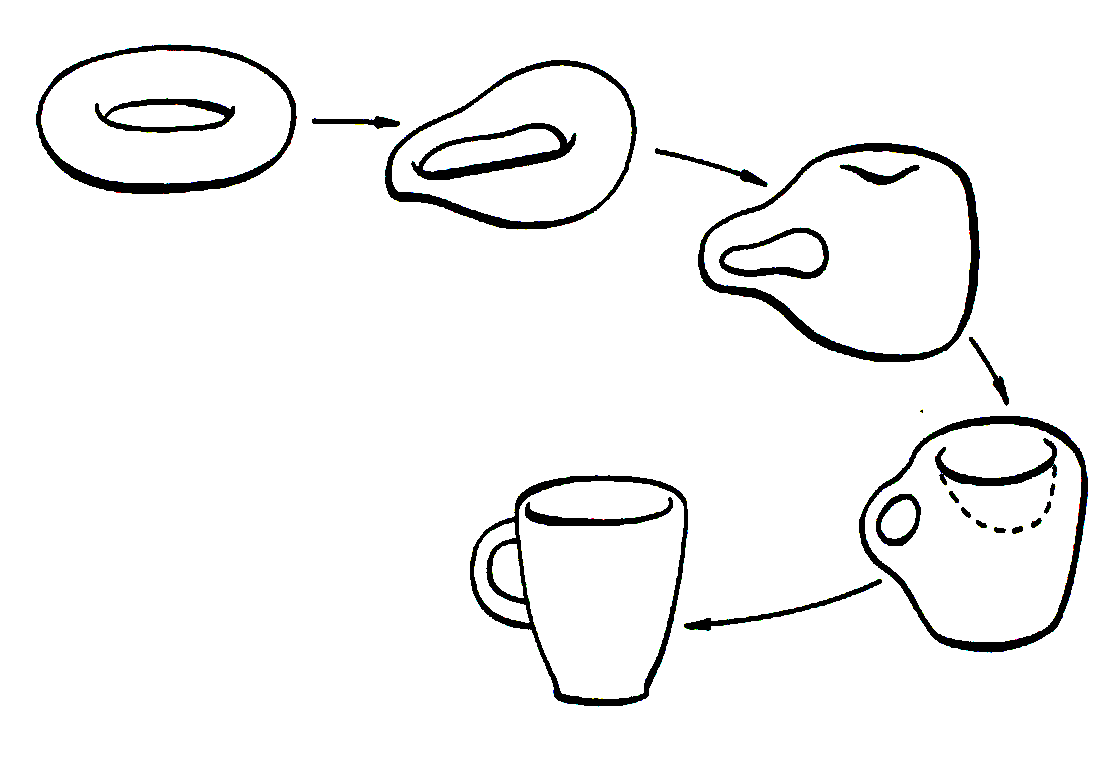
\includegraphics[height=0.65\textwidth]{mugtopology.png}
        
    \end{column}
\end{columns}
}

\frame{
  \frametitle{Topological insulators}
  \begin{itemize}
    \item The vacuum has the simplest band
    structure.

    \item Insulators are `conventional' or
    `topologically trivial'
    if a homeomorphism of lattice
    parameters can transform the
    band structure into the band structure of
    the vacuum.

    \item In quantum mechanics, adiabatic processes are gradual changes in parameters
      which make eigenstates evolve continuously.

    \item Conventional insulators are adiabatically
    connected to the `atomic limit'.

    \item Not all materials are topologically trivial!

  \end{itemize}

}

\frame{
  \frametitle{Berry phase \& Electronic structure}
  \begin{itemize}
   
  \item The Berry phase is the change in phase picked up by the wavefunction
    upon completing an adiabatic loop in the Brillouin zone.
  
  \end{itemize}
  
  \begin{block}{Berry phase}
  \begin{equation}
    \phi = \oint_C{d\boldsymbol{\lambda}\cdot i\braket{u_{\bm{k}}|\nabla_{\!\bm{k}}|u_{\bm{k}} } }
    =\oint_C{d\boldsymbol{\lambda}\cdot \bm{A} }.
  \end{equation}
  \end{block}

  \begin{itemize}

  \item In quantum mechanics phases are unphysical; only phase differences are observable, so
    the system is underdetermined by a Berry phase.

  \item This is analogous to gauge freedom in electromagnetism and the Berry potential
    has a gauge transformation similar to the electromagnetic 
    four-potential.
  \end{itemize}



}



\frame{
  \frametitle{Berry Phase \& Electronic structure}
 
  \begin{alertblock}{Chern theorem}
  \begin{equation}
    \Phi = \iint_{\Sigma}{d\bm{S}\cdot \overrightarrow{\nabla}\!\times\!\bm{A}} = 2\pi c \, ;
    \quad c\in \mathbb{Z} 
  \end{equation}
  \end{alertblock}


  \begin{itemize}
  
    \item The Chern theorem tells us that the Berry flux through a surface in the Brillouin 
      zone is a topologically invariant integer multiple of $2\pi$.
    \item Additionally, electronic band degeneracy points are monopoles of Berry flux and are
      thus topologically protected.
  \end{itemize}
}


\frame{
  \frametitle{Dirac \& Weyl semimetals}
  
    \begin{itemize}
      \item Weyl semimetals (WSMs) are materials with linear dispersion, given by the Weyl Hamiltonian,
        at band degeneracies near the fermi energy called Weyl points.
      \item Weyl points have Chern numbers of $c = \pm 1$; positive and negative chirality.
      
    \end{itemize}
    
    \begin{block}{Weyl point symmetries}
      \centering
      Inversion symmetry $\implies \boldsymbol{\Omega}(-\bm{k}) = - \boldsymbol{\Omega}(\bm{k})$. \\
      Time-reversal symmetry $\implies \boldsymbol{\Omega}(-\bm{k}) = \boldsymbol{\Omega}(\bm{k})$.
    \end{block}


    \begin{itemize}
    \item Dirac semimetals (DSMs) are WSMs which have both inversion and time-reversal
        symmetry leading to band crossings being four overlapping Weyl points (Dirac points).
  
    \end{itemize}

}


\frame{
  \frametitle{Dirac \& Weyl semimetals}
  \begin{columns}

    \begin{column}{0.55\textwidth}
    \begin{itemize}
    
    \item The most famous 2D DSM is graphene which has 6 Dirac points at the edge of the
      Brillouin zone.

    \item The Hamiltonian is the massless Dirac Hamiltonian; thus, quasiparticles in graphene
      are observed as massless Dirac fermions~\cite{DiracFerm}.

    \item This suggests WSM quasiparticles should exhibit the effects of relativistic 
      Weyl fermions. In particular, the chiral anomaly.

    \end{itemize}
    \end{column}


  \begin{column}{0.5\textwidth}
    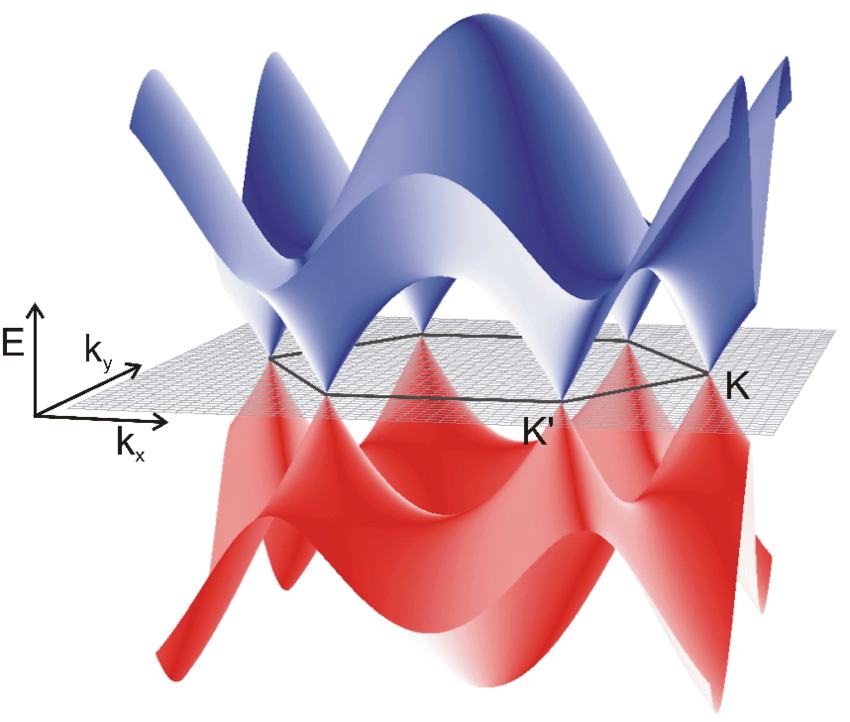
\includegraphics[width=0.9\textwidth]{GrapheneDispersion.png}~\cite{graphene}
  \end{column}


\end{columns}

}


\frame{
  \frametitle{What is an anomaly?}

  \begin{itemize}
    \item An anomaly is a symmetry of a classical theory which is broken in the 
      associated quantum field theory.
    \item Noether's theorem tells us that symmetries correspond to physical conservation 
      laws.
    \item Thus, an anomaly can be seen as the existence of quantum processes which violate
      a classical conservation law.
  \end{itemize}
}


\frame{
  \frametitle{The Chiral Anomaly}
  
  \begin{itemize}

  \item The Dirac equation has two symmetries which correspond to two conserved currents; 
    the axial and vector currents ($j \, \& \, j_5$).

  \item The vector current is the sum of the currents of opposite chirality whereas
    the axial current is the difference.

  \item The axial symmetry is anomalous; the axial current is not conserved.
   
  \end{itemize}

  
  \begin{alertblock}{Chiral anomaly}
    \begin{equation}
      \overrightarrow{\nabla}\cdot j_5 = \frac{e^2}{4\pi^2\hbar^2}\bm{E}\cdot\bm{B}
    \end{equation}
  \end{alertblock}
 
}

\frame{
  \frametitle{The Chiral Anomaly}


  \begin{columns}


  \begin{column}{0.55\textwidth}
  \begin{itemize}
    \item In high energy physics, the chiral anomaly manifests as the fast $\pi^0$ decay rate
      called the Adler–Bell–Jackiw anomaly~\cite{Adler,JackiwBell}.
    \item In WSMs the chiral anomly is observed as a large negative magnetoresistance 
      as the external fields cause electrons to flow between Weyl points of 
      opposite chirality.
  \end{itemize}
  \end{column}

  \begin{column}{0.5\textwidth}
    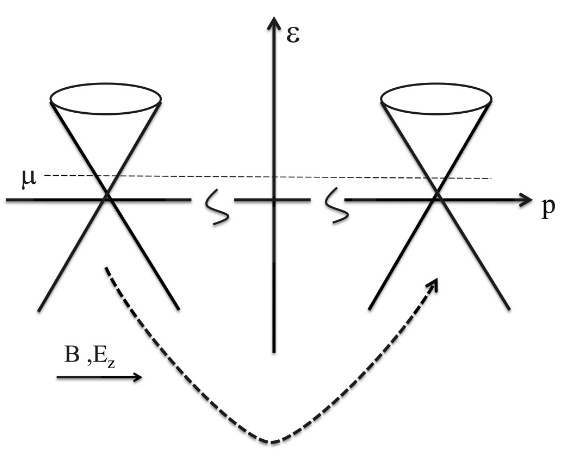
\includegraphics[width=\textwidth]{Chiral.png}~\cite{SonSpivak}
  \end{column}

  \end{columns}
}


\frame{
  \frametitle{Experiments}
  
  \begin{columns}

  \begin{column}{0.6\textwidth}
  \begin{itemize}
    \item TaAs was the first WSM discovered and exhibits a weak negative linear 
      magnetoresistance (LMR)~\cite{TaAs}. 
    \item However, the high carrier mobility of
      TaAs and other WSMs produces current jetting which also create negative LMRs~\cite{Squeezetest}.

  \end{itemize}
  \end{column}

  \begin{column}{0.4\textwidth}
    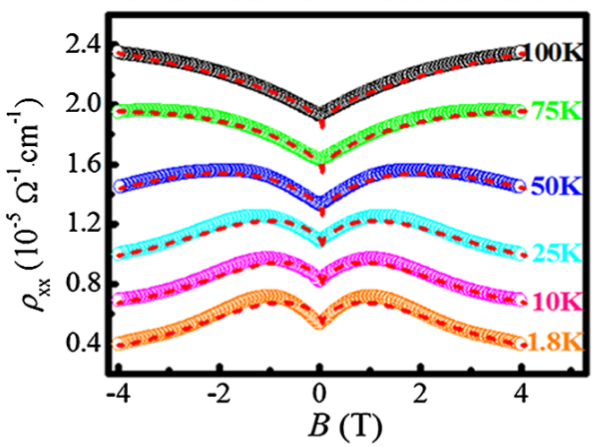
\includegraphics[width=\textwidth]{TaAs.png}
  \end{column}


  \end{columns}
}

\frame{
  \frametitle{Experiments}
  \begin{columns}

  \begin{column}{0.55\textwidth}
  
    \begin{itemize}
      \item The Na$_3$Bi is a DSM however, an external $\bm{B}$ field breaks 
        the time-reversal symmetry splitting the two Dirac points into
        Weyl points\cite{Na3Bi}.
      \item Moreover, the low carrier mobility excludes current jetting effects
        making the negative LMR in Na$_3$Bi the strongest evidence for the 
        chiral anomaly in condensed matter.
    \end{itemize}

  \end{column}

  \begin{column}{0.5\textwidth}
    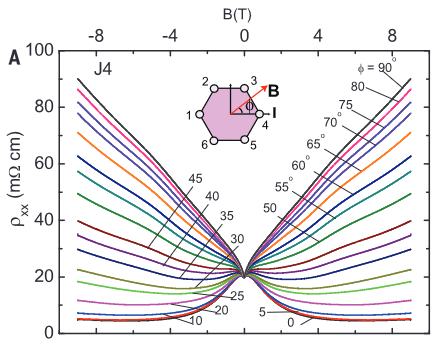
\includegraphics[width=\textwidth]{Na3Bi.png}
  \end{column}


  \end{columns}

}


\frame{
  \frametitle{References}
  \bibliography{refs.bib}
}








\end{document}
